\documentclass[tikz,border=12pt]{standalone}
\usepackage{helvet}
\usepackage{amsmath,amssymb}
\renewcommand{\familydefault}{\sfdefault}
\usepackage{tikz}
\usepackage{tikz-3dplot}
\usetikzlibrary{shapes.geometric, calc, positioning, decorations.pathmorphing, decorations.markings, arrows.meta}

\definecolor{emeraldpine}{HTML}{1A4D3E}
\definecolor{harvardcrimson}{HTML}{A51C30}
\definecolor{ethdarkblue}{HTML}{1F407A}
\definecolor{ethpetrol}{HTML}{007A87}
\definecolor{ethbronze}{HTML}{B87333}
\definecolor{ink}{HTML}{1A202C}
\definecolor{cardbg}{HTML}{F8FAFC}
\definecolor{paleink}{HTML}{94A3B8}

\begin{document}
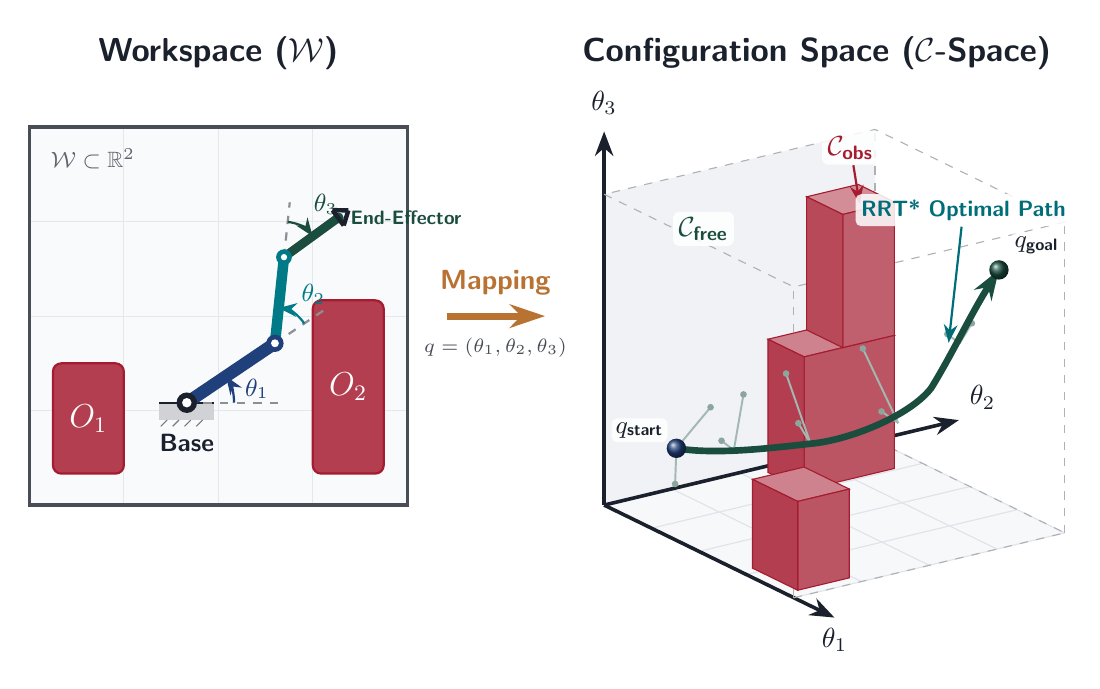
\begin{tikzpicture}[font=\sffamily, >=Stealth]

% ==========================================
% 1. 2D WORKSPACE ON THE LEFT
% ==========================================
\begin{scope}[shift={(0,0)}]
    % Title
    \node[anchor=south, font=\large\bfseries, text=ink] at (2.4,5.4) {Workspace ($\mathcal{W}$)};
    
    % Workspace boundary
    \fill[cardbg] (0,0) rectangle (4.8,4.8);
    \draw[step=1.2, paleink!25, thin] (0,0) grid (4.8,4.8);
    \draw[line width=1.2pt, ink!80] (0,0) rectangle (4.8,4.8);
    
    % Coordinate label
    \node[anchor=north west, font=\footnotesize\bfseries, text=ink!70] at (0.15, 4.65) {$\mathcal{W} \subset \mathbb{R}^2$};
    
    % Obstacle O_1 (bottom-left)
    \filldraw[fill=harvardcrimson!85, draw=harvardcrimson, thick, rounded corners=3pt] 
        (0.3,0.4) rectangle (1.2,1.8);
    \node[white, font=\bfseries\large] at (0.75,1.1) {$O_1$};
    
    % Obstacle O_2 (right side)
    \filldraw[fill=harvardcrimson!85, draw=harvardcrimson, thick, rounded corners=3pt] 
        (3.6,0.4) rectangle (4.5,2.6);
    \node[white, font=\bfseries\large] at (4.05,1.5) {$O_2$};
    
    % Robot base mount (centered at x=2.0)
    \coordinate (base) at (2.0, 1.3);
    \fill[ink!20] ($(base)+(-0.35,-0.22)$) rectangle ($(base)+(0.35,0)$);
    \draw[thick, ink] ($(base)+(-0.35,0)$) -- ($(base)+(0.35,0)$);
    \foreach \hx in {-0.25, -0.1, 0.05, 0.2} {
        \draw[thin, ink!60] ($(base)+(\hx,-0.22)$) -- ($(base)+(\hx-0.08,-0.3)$);
    }
    
    % Kinematics for 3-link arm
    \coordinate (j2) at ($(base) + (34:1.35)$);
    \coordinate (j3) at ($(j2) + (84:1.1)$);
    \coordinate (ee) at ($(j3) + (36:0.85)$);
    
    % Angle 1 reference & arc
    \draw[dashed, ink!50, thick] (base) -- +(1.2,0);
    \draw[->, thick, ethdarkblue] (base) ++(0:0.6) arc (0:34:0.6) node[midway, right=1pt, font=\small\bfseries] {$\theta_1$};
    
    % Angle 2 reference & arc
    \draw[dashed, ink!50, thick] (j2) -- +(34:0.75);
    \draw[->, thick, ethpetrol] (j2) ++(34:0.45) arc (34:84:0.45) node[midway, above right=-1pt, font=\small\bfseries] {$\theta_2$};
    
    % Angle 3 reference & arc
    \draw[dashed, ink!50, thick] (j3) -- +(84:0.7);
    \draw[<-, thick, emeraldpine] (j3) ++(36:0.45) arc (36:84:0.45) node[midway, above right=1pt, font=\small\bfseries] {$\theta_3$};
    
    % Links
    \draw[line width=4.5pt, ethdarkblue, line cap=round] (base) -- (j2);
    \draw[line width=3.8pt, ethpetrol, line cap=round] (j2) -- (j3);
    \draw[line width=3.2pt, emeraldpine, line cap=round] (j3) -- (ee);
    
    % Joint circles
    \fill[ink] (base) circle (0.13);
    \fill[white] (base) circle (0.06);
    \node[below=8pt, font=\small\bfseries, text=ink] at (base) {Base};
    
    \fill[ethdarkblue] (j2) circle (0.11);
    \fill[white] (j2) circle (0.05);
    
    \fill[ethpetrol] (j3) circle (0.10);
    \fill[white] (j3) circle (0.04);
    
    % End effector gripper
    \fill[emeraldpine] (ee) circle (0.07);
    \draw[line width=1.6pt, ink] ($(ee)+(126:0.12)$) -- ($(ee)+(306:0.12)$);
    \draw[line width=1.6pt, ink] ($(ee)+(126:0.12)$) -- ($(ee)+(36:0.16)$);
    \draw[line width=1.6pt, ink] ($(ee)+(306:0.12)$) -- ($(ee)+(36:0.16)$);
    \node[above=3pt, right=1pt, font=\scriptsize\bfseries, text=emeraldpine] at (ee) {End-Effector};

\end{scope}

% ==========================================
% 2. MAPPING ARROW IN THE MIDDLE
% ==========================================
\begin{scope}[shift={(4.8, 0)}]
    \draw[-{Stealth[length=4.5mm, width=3mm]}, line width=2.5pt, ethbronze] (0.5, 2.4) -- (1.75, 2.4);
    \node[anchor=south, font=\normalsize\bfseries, text=ethbronze] at (1.12, 2.55) {Mapping};
    \node[anchor=north, font=\scriptsize\sffamily, text=ink!80] at (1.12, 2.25) {$q = (\theta_1,\theta_2,\theta_3)$};
\end{scope}

% ==========================================
% 3. 3D CONFIGURATION SPACE ON THE RIGHT
% ==========================================
\tdplotsetmaincoords{70}{55}
\begin{scope}[shift={(7.3, 0.0)}, tdplot_main_coords]
    \def\L{4.2}
    
    % Shaded back walls for 3D depth perception
    \fill[paleink!8] (0,0,0) -- (\L,0,0) -- (\L,\L,0) -- (0,\L,0) -- cycle;
    \fill[paleink!14] (0,0,0) -- (0,\L,0) -- (0,\L,\L) -- (0,0,\L) -- cycle;
    
    % Grid lines on floor
    \foreach \t in {1.05, 2.1, 3.15, 4.2} {
        \draw[paleink!30, thin] (\t,0,0) -- (\t,\L,0);
        \draw[paleink!30, thin] (0,\t,0) -- (\L,\t,0);
    }
    
    % Coordinate axes at origin
    \draw[->, line width=1.3pt, ink] (0,0,0) -- (\L+0.9,0,0) node[anchor=north, font=\normalsize\bfseries]{$\theta_1$};
    \draw[->, line width=1.3pt, ink] (0,0,0) -- (0,\L+1.3,0) node[anchor=south west, font=\normalsize\bfseries]{$\theta_2$};
    \draw[->, line width=1.3pt, ink] (0,0,0) -- (0,0,\L+0.85) node[anchor=south, font=\normalsize\bfseries, yshift=2pt]{$\theta_3$};
    
    % Wireframe ceiling and outer walls
    \draw[dashed, ink!35, thin] (0,0,\L) -- (\L,0,\L) -- (\L,\L,\L) -- (0,\L,\L) -- cycle;
    \draw[dashed, ink!35, thin] (\L,0,0) -- (\L,0,\L);
    \draw[dashed, ink!35, thin] (0,\L,0) -- (0,\L,\L);
    \draw[dashed, ink!35, thin] (\L,\L,0) -- (\L,\L,\L);
    \draw[dashed, ink!35, thin] (\L,0,0) -- (\L,\L,0) -- (0,\L,0);

    % ----------------------------------------------------
    % NON-CONVEX C-SPACE OBSTACLE 1 (Mapped from O_1)
    % Placed at back-left: y in [2.4, 3.8], x in [0.2, 1.0]
    % ----------------------------------------------------
    % Lower part of Obs 1
    \filldraw[fill=harvardcrimson!55, draw=harvardcrimson, thin] 
        (0.2, 2.4, 1.8) -- (1.0, 2.4, 1.8) -- (1.0, 3.8, 1.8) -- (0.2, 3.8, 1.8) -- cycle; % top
    \filldraw[fill=harvardcrimson!75, draw=harvardcrimson, thin] 
        (1.0, 2.4, 0.0) -- (1.0, 3.8, 0.0) -- (1.0, 3.8, 1.8) -- (1.0, 2.4, 1.8) -- cycle; % right
    \filldraw[fill=harvardcrimson!85, draw=harvardcrimson, thin] 
        (0.2, 2.4, 0.0) -- (1.0, 2.4, 0.0) -- (1.0, 2.4, 1.8) -- (0.2, 2.4, 1.8) -- cycle; % front

    % Upper tower of Obs 1 (concave step): y in [3.0, 3.8], x in [0.2, 1.0], z in [1.8, 3.6]
    \filldraw[fill=harvardcrimson!50, draw=harvardcrimson, thin] 
        (0.2, 3.0, 3.6) -- (1.0, 3.0, 3.6) -- (1.0, 3.8, 3.6) -- (0.2, 3.8, 3.6) -- cycle; % top
    \filldraw[fill=harvardcrimson!70, draw=harvardcrimson, thin] 
        (1.0, 3.0, 1.8) -- (1.0, 3.8, 1.8) -- (1.0, 3.8, 3.6) -- (1.0, 3.0, 3.6) -- cycle; % right
    \filldraw[fill=harvardcrimson!80, draw=harvardcrimson, thin] 
        (0.2, 3.0, 1.8) -- (1.0, 3.0, 1.8) -- (1.0, 3.0, 3.6) -- (0.2, 3.0, 3.6) -- cycle; % front

    % ----------------------------------------------------
    % C-SPACE OBSTACLE 2 (Mapped from O_2)
    % Placed at front-right: x in [3.0, 4.0], y in [0.2, 1.0], z in [0, 1.2]
    % ----------------------------------------------------
    \filldraw[fill=harvardcrimson!55, draw=harvardcrimson, thin] 
        (3.0, 0.2, 1.2) -- (4.0, 0.2, 1.2) -- (4.0, 1.0, 1.2) -- (3.0, 1.0, 1.2) -- cycle; % top
    \filldraw[fill=harvardcrimson!75, draw=harvardcrimson, thin] 
        (4.0, 0.2, 0.0) -- (4.0, 1.0, 0.0) -- (4.0, 1.0, 1.2) -- (4.0, 0.2, 1.2) -- cycle; % right
    \filldraw[fill=harvardcrimson!85, draw=harvardcrimson, thin] 
        (3.0, 0.2, 0.0) -- (4.0, 0.2, 0.0) -- (4.0, 0.2, 1.2) -- (3.0, 0.2, 1.2) -- cycle; % front

    % ----------------------------------------------------
    % RRT* EXPLORATION TREE IN C_free
    % ----------------------------------------------------
    \coordinate (qstart) at (0.6, 0.7, 0.8);
    \coordinate (qgoal) at (3.6, 3.6, 3.5);
    
    % Free corridor waypoints
    \coordinate (p1) at (1.3, 1.1, 0.9);
    \coordinate (p2) at (2.0, 1.8, 1.05);
    \coordinate (p3) at (2.8, 2.6, 1.4);
    \coordinate (p4) at (3.3, 3.2, 2.5);
    
    % Faint RRT* exploration branches
    \draw[emeraldpine!40, line width=0.7pt] (qstart) -- (0.5, 1.3, 1.2);
    \draw[emeraldpine!40, line width=0.7pt] (qstart) -- (1.0, 0.4, 0.5);
    \draw[emeraldpine!40, line width=0.7pt] (p1) -- (0.8, 1.6, 1.4);
    \draw[emeraldpine!40, line width=0.7pt] (p1) -- (1.6, 0.7, 1.2);
    \draw[emeraldpine!40, line width=0.7pt] (p2) -- (1.6, 1.7, 1.9);
    \draw[emeraldpine!40, line width=0.7pt] (p2) -- (2.3, 1.4, 1.5);
    \draw[emeraldpine!40, line width=0.7pt] (p3) -- (2.3, 2.4, 2.3);
    \draw[emeraldpine!40, line width=0.7pt] (p3) -- (3.0, 2.2, 1.7);
    \draw[emeraldpine!40, line width=0.7pt] (p4) -- (3.6, 2.8, 2.8);
    \draw[emeraldpine!40, line width=0.7pt] (p4) -- (3.0, 3.6, 2.6);
    
    % Sampled tree nodes
    \foreach \coord in {(0.5, 1.3, 1.2), (1.0, 0.4, 0.5), (0.8, 1.6, 1.4), (1.6, 0.7, 1.2), (1.6, 1.7, 1.9), (2.3, 1.4, 1.5), (2.3, 2.4, 2.3), (3.0, 2.2, 1.7), (3.6, 2.8, 2.8), (3.0, 3.6, 2.6)} {
        \fill[emeraldpine!50] \coord circle (1.2pt);
    }
    
    % Optimal RRT* path (smooth continuous spline winding through corridor)
    \draw[emeraldpine, line width=2.4pt, -{Stealth[length=3.8mm, width=2.6mm]}] 
        (qstart) .. controls (1.2, 0.9, 0.85) and (1.6, 1.4, 0.95) .. 
        (p2) .. controls (2.4, 2.1, 1.15) and (2.9, 2.7, 1.5) .. 
        (3.1, 2.9, 1.9) .. controls (3.3, 3.1, 2.4) and (3.4, 3.3, 2.9) .. 
        (qgoal);

    % Start and Goal nodes (prominent spheres)
    \shade[ball color=ethdarkblue] (qstart) circle (3.5pt) 
        node[anchor=south east, font=\small\bfseries, text=ink, fill=white, fill opacity=0.85, text opacity=1, inner sep=1.5pt, rounded corners=2pt, xshift=-3pt, yshift=2pt] {$q_{\text{start}}$};
        
    \shade[ball color=emeraldpine] (qgoal) circle (3.5pt) 
        node[anchor=south west, font=\small\bfseries, text=ink, fill=white, fill opacity=0.85, text opacity=1, inner sep=1.5pt, rounded corners=2pt, xshift=4pt, yshift=4pt] {$q_{\text{goal}}$};
        
    % Annotations
    \node[harvardcrimson, font=\sffamily\bfseries, fill=white, fill opacity=0.85, text opacity=1, inner sep=2pt, rounded corners=2pt] 
        (cobs_lbl) at (0.6, 3.4, 4.3) {$\mathcal{C}_{\text{obs}}$};
    \draw[harvardcrimson, thick, ->] (cobs_lbl) -- (0.8, 3.4, 3.6);
    
    \node[emeraldpine, font=\sffamily\bfseries, fill=white, fill opacity=0.85, text opacity=1, inner sep=2pt, rounded corners=2pt] 
        (cfree_lbl) at (0.2, 1.4, 3.5) {$\mathcal{C}_{\text{free}}$};
        
    % RRT* optimal path label placed in open space above climbing path
    \node[ethpetrol!90!black, font=\footnotesize\bfseries, fill=white, fill opacity=0.85, text opacity=1, inner sep=2pt, rounded corners=2pt] 
        (rrt_lbl) at (3.1, 3.4, 4.2) {RRT* Optimal Path};
    \draw[ethpetrol!90!black, thick, ->] (rrt_lbl) -- (3.2, 3.1, 2.5);

\end{scope}

\node[anchor=south, font=\large\bfseries, text=ink] at (10.0,5.4) {Configuration Space ($\mathcal{C}$-Space)};

\end{tikzpicture}
\end{document}
